\section{Problem Statement} \label{ICRA:sec:problem_statement}

The problem addressed in this paper is to adapt a dynamics model trained in a source environment to data collected in a target environment, where the source and target environments have dynamics which are similar in some regions of the state-action space, but different in others. Furthermore, we consider the case where data collection is done by planning and executing paths to goals in the target environment using the learned dynamics model.

To formalize this, first consider the standard dynamics learning problem with a dataset $\dataset$ of transitions of states, actions, and next states $\transition$. We also assume a distance function $\distf{\state_1}{\state_2}$ that returns a scalar is given. The true dynamics are $\state'=\dynamics(\state,\action)$, and the learned dynamics are $\pred{\state}'=\learnedDynamics(\state,\action)$. We propose defining the source and target environment dynamics as similar for a transition if $\distf{\sourceDynamics(\state,\action)}{\targetDynamics(\state,\action)} < \softFilteringThrehsold$. The threshold $\softFilteringThrehsold$ should be small enough that it excludes distracting transitions, but large enough to include as much data from the target environment as possible. Let $\DST$ be the set of transitions from the target environment where this similarity condition holds.

In order to minimize the amount of data needed for adaptation to generalize, we aim to adapt the dynamics only to transitions from regions where this similarity condition holds ($\DST$). However, we also care about successfully completing the task, and therefore we also assume there are paths $\traj$ to the goal $\state^T\in\goal$ within the regions of similar dynamics $(\state^t,\action^t,\state^{t+1}) \in \DST $.

While the ultimate objective of adaptation should be to maximize task success in the target environment, an important condition for task success is minimizing prediction error on $\DST$. If the goal is reachable within $\DST$ (as we assume), the prediction error on $\DST$ is small (our objective), and our motion planner is constrained to stay in $\DST$, then we can also expect high task success. Next, we discuss how our adaptation method minimizes error on $\DST$, followed by how we can achieve high task success by additionally constraining a motion planner to $\DST$.

\begin{figure}
    \centering
    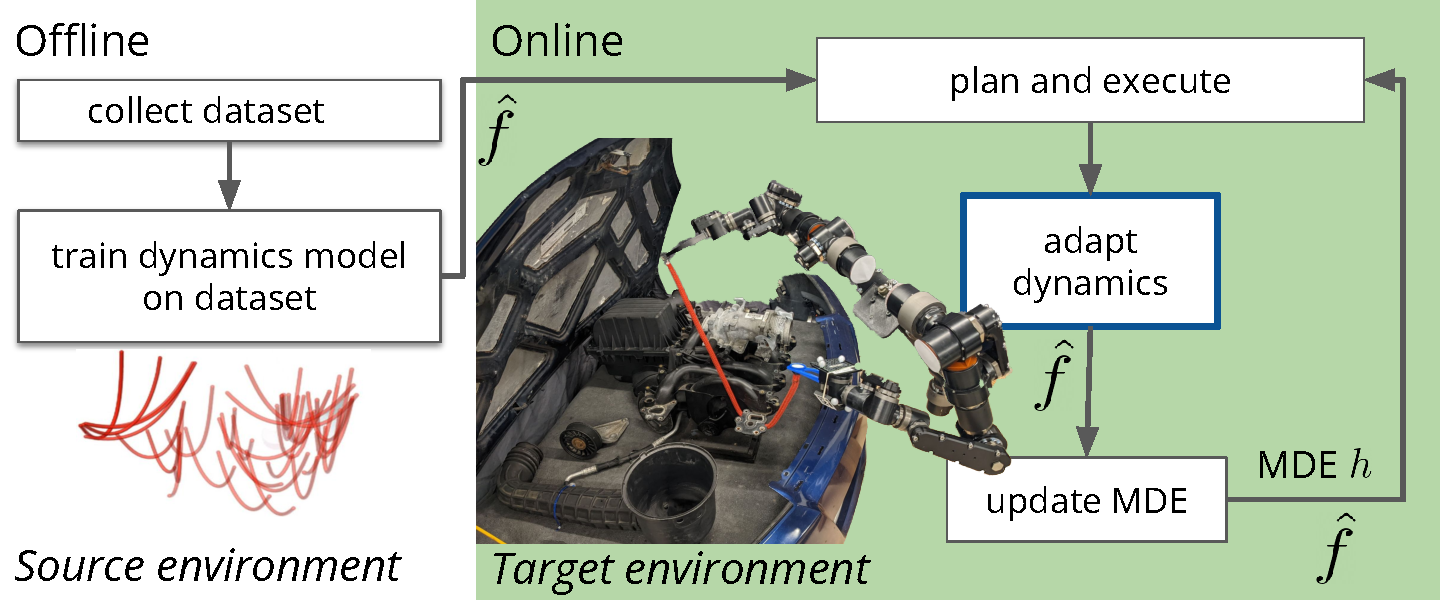
\includegraphics[width=1\linewidth]{Chap4/images/overview_diagram.pdf}
    \caption{Block diagram showing the steps of our full online adaptation method. A dynamics model is initialized offline in the source environment (left), then adapted online in the target environment.}
    \label{ICRA:fig:diagram}
\end{figure}
